\chapter{程序编写}
\label{cha:Program}

\section{VS Code下Arduino编程环境配置}

VS Code下Arduino编程环境配置\footnote{\url{https://docs.microsoft.com/zh-cn/azure/iot-hub/iot-hub-arduino-iot-devkit-az3166-get-started}}
方法如下:

\begin{enumerate}

    \item
        安装 \href{https://www.arduino.cc/en/Main/Software}{Arduino IDE}。此IDE 提供必要的工具链用于编译和上传 Arduino 代码。
        
        \begin{itemize}
        \item
            \textbf{Windows}:使用 Windows Installer 版本,不要从应用商店安装。
        \item
            \textbf{macOS}:将解压缩的 \textbf{Arduino.app} 拖放到\texttt{/Applications} 文件夹中。
        \item
            \textbf{Ubuntu}:解压缩到某个文件夹中,例如 \texttt{\$HOME/Downloads/arduino-1.8.8}
        \end{itemize}
    \item
         安装\href{https://code.visualstudio.com/}{Visual Studio Code}是一个跨平台源代码编辑器,其中包含功能强大的intellisense、代码完成和调试支持以及可从 marketplace 安装丰富的扩展。
    \item
        启动 VS Code,在扩展市场中找到 \textbf{Arduino} 并安装它。此扩展提供在 Arduino 平台上进行开发的增强体验。
    \item
        为 VS Code 配置 Arduino 设置。
        
        在 Visual Studio Code 中,单击 "\textbf{文件" \textgreater{} 首选项 \textgreater{} 设置}(在 macOS 上,\textbf{代码 \textgreater{} 首选项 \textgreater{} 设置})。 然后单击 "\emph{设置}" 页右上角的 "\textbf{打开设置(JSON)} " 图标。

        根据你的平台添加以下行来配置 Arduino:
    
        \textbf{Windows}:
        \begin{tcolorbox}
            "arduino.path": "C:\textbackslash{}\textbackslash{}Program Files (x86)\textbackslash{}\textbackslash{}Arduino",
        \end{tcolorbox}

        \textbf{macOS}:
    
        \begin{tcolorbox}    
            "arduino.path": "/Applications",
        \end{tcolorbox}

        \textbf{Ubuntu}:
    
        将下面的 \textbf{\{username\}} 占位符替换为你的用户名。
        \begin{tcolorbox}
            "arduino.path": "/home/\{username\}/Downloads/arduino-1.8.8",
        \end{tcolorbox}
    \end{enumerate}



\section{TB6612电机测试程序}

在引脚分配时,我们将两片TB6612连接在Mega2560上。

四个PWM调速信号输出引脚由能输出PWM波的PH 3 4 5 6承担,分别接到PWM A B C D,在Arduino IDE程序中对应 Digital pin 6 7 8 9 (PWM)。

每个电机控制的IN1 IN2 分别由 PA0-PA7 8个引脚承担,对应Digital pin 22 - 29,由于只是使能信号,普通数字引脚即可,不需要特定的PWM引脚。

STBY信号由 PG2 ( ALE ) Digital pin 39统一给出,即所有电机统一使能或待机。

\section{WS2812B测试程序}

由PE5 ( OC3C/INT5 ) Digital pin 3 (PWM) 引脚提供串行通信信号。

需要在Arduino IDE 安装Adafruit NeoPixel库,直接通过Library Manager安装即可,如图~\ref{fig:Adafruit-NeoPixel-Installation}。

\begin{figure}[htbp]
    \centering
    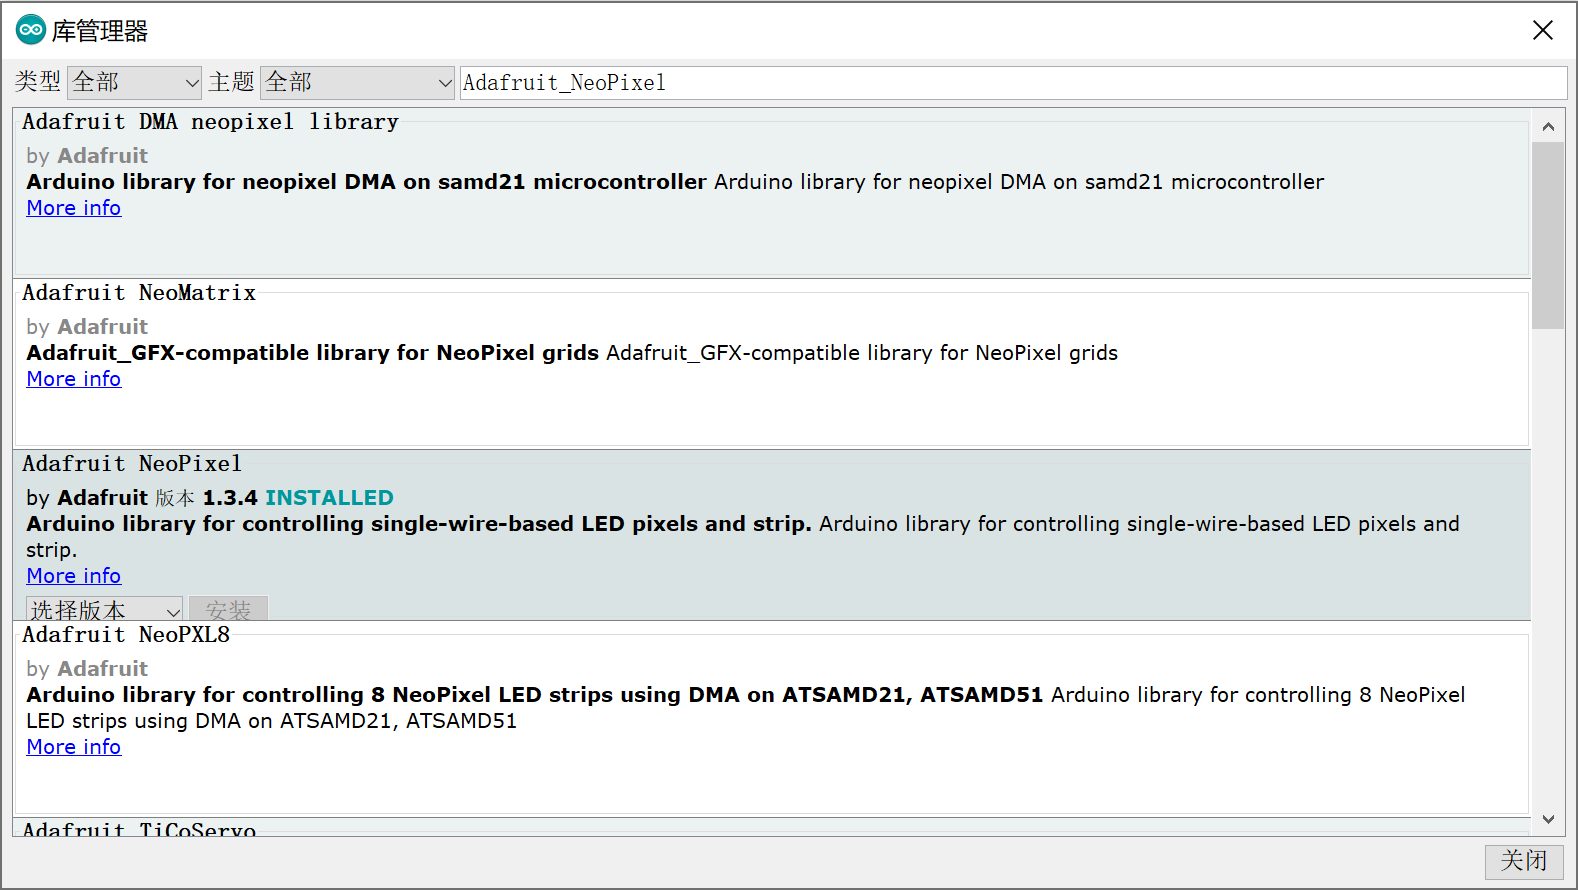
\includegraphics[width=\textwidth]{Adafruit-NeoPixel-Installation.png}
    \caption{通过Library Manager安装Adafruit NeoPixel库}
    \label{fig:Adafruit-NeoPixel-Installation}
\end{figure}

本项目测试程序在原有Adafruit NeoPixel库示例程序strandtest上修改而成,可以让9个RGB LED以各种规律发光以测试功能的完备性。


\section{ESP32}

在Arduino IDE内也可以添加对ESP32 Boards的支持,在Arduino IDE设置里的"Additional Board Manager URLs"中添加\url{https://raw.githubusercontent.com/espressif/arduino-esp32/gh-pages/package_esp32_index.json} 以英文逗号和其他网址分隔,之后在Tools > Board > Boards Manager… 内安装 "ESP32 by Espressif Systems"即可。Arduino core for the ESP32也可以在\url{https://github.com/espressif/arduino-esp32}下载源码自己编译。